\documentclass[11pt]{article}

\usepackage[a4paper,margin=1in]{geometry}
\usepackage{graphicx}
\usepackage{pdflscape}
\usepackage{float}
\usepackage{booktabs}
\usepackage{enumitem}
\usepackage{amsmath}
\usepackage{fancyhdr}
\usepackage{lastpage}
\usepackage{titlesec}
\usepackage[T1]{fontenc}
\usepackage{lmodern}

\pagestyle{fancy}
\fancyhf{}
\fancyhead[L]{Kyle Strother}
\fancyhead[C]{ACIT4420}
\fancyhead[R]{BusBidder Spain}
\fancyfoot[C]{Page \thepage\ of \pageref{LastPage}}
\renewcommand{\headrulewidth}{0.4pt}
\renewcommand{\footrulewidth}{0.4pt}

\setlength{\parskip}{0.5em}
\setlength{\parindent}{0pt}
\setlength{\headheight}{14pt}
\setlist[itemize]{leftmargin=1.5em}

\begin{document}

\begin{titlepage}
    \centering
    \vspace*{2cm}

    {\LARGE \textbf{BusBidder Spain: Personalized Bus Journey Comparison and Booking System}\par}
    \vspace{1.5cm}

    {\large Kyle Strother\par}
    \vspace{0.5cm}

    {\large \today\par}

    \vfill
\end{titlepage}

\tableofcontents
\newpage

\section{Introduction}
BusBidder is a bus-booking marketplace that allows users to compare offers
from five bus companies. It tries to simplify journey selection by
filtering unsuitable offers and ranking the remaining options based on user's priorities.

Comparing bus offers is difficult because the cheapest ticket isn't necessarily the best choice.
Differences in duration, departure times, transfers, and flexibility
can affect an offer's value to a user. Few users agree on what matters most for a trip.

BusBidder's objective is to provide personalised filtering and a weighted ranking system, that'll help
travellers identify the most suitable journey based on their requirements and priorities.

\section{Requirements and Problem Interpretation}

The application functions by:
\begin{itemize}[nosep]
\item loading/validating Trip data
\item removing Trips that don't meet hard constraints
\item scoring remaining offers using a weighted ranking model set by individual users
\item presenting explainable recommendations
\item supporting simulated bookings for multiple users
\end{itemize}

The application uses a modular, object-oriented Python design to separate functional responsibilities
such as data management, validation, filtering, scoring, and booking.
A weighted scoring model allows different criteria to be normalised and combined into a measurable score.
This scoring and its composition is created in a way that is accessible and referencable outside of internal objects to allow
explanation of ranking to users.

A consideration in this application's design is Hard versus Soft Constraints.
Hard constraints determine whether an offer is acceptable and
can be set by the user on any field such as destination, travel dates, budget, and seat availability.
Preferences/Priorities, such as lower prices, shorter journeys, and ticket flexibility,
are Soft constraints set by the user and only influence the ranking.


\newpage
\section{System Architecture and Software Design}
\subsection{Data Flow Diagram}
\begin{figure}[H]
\centering
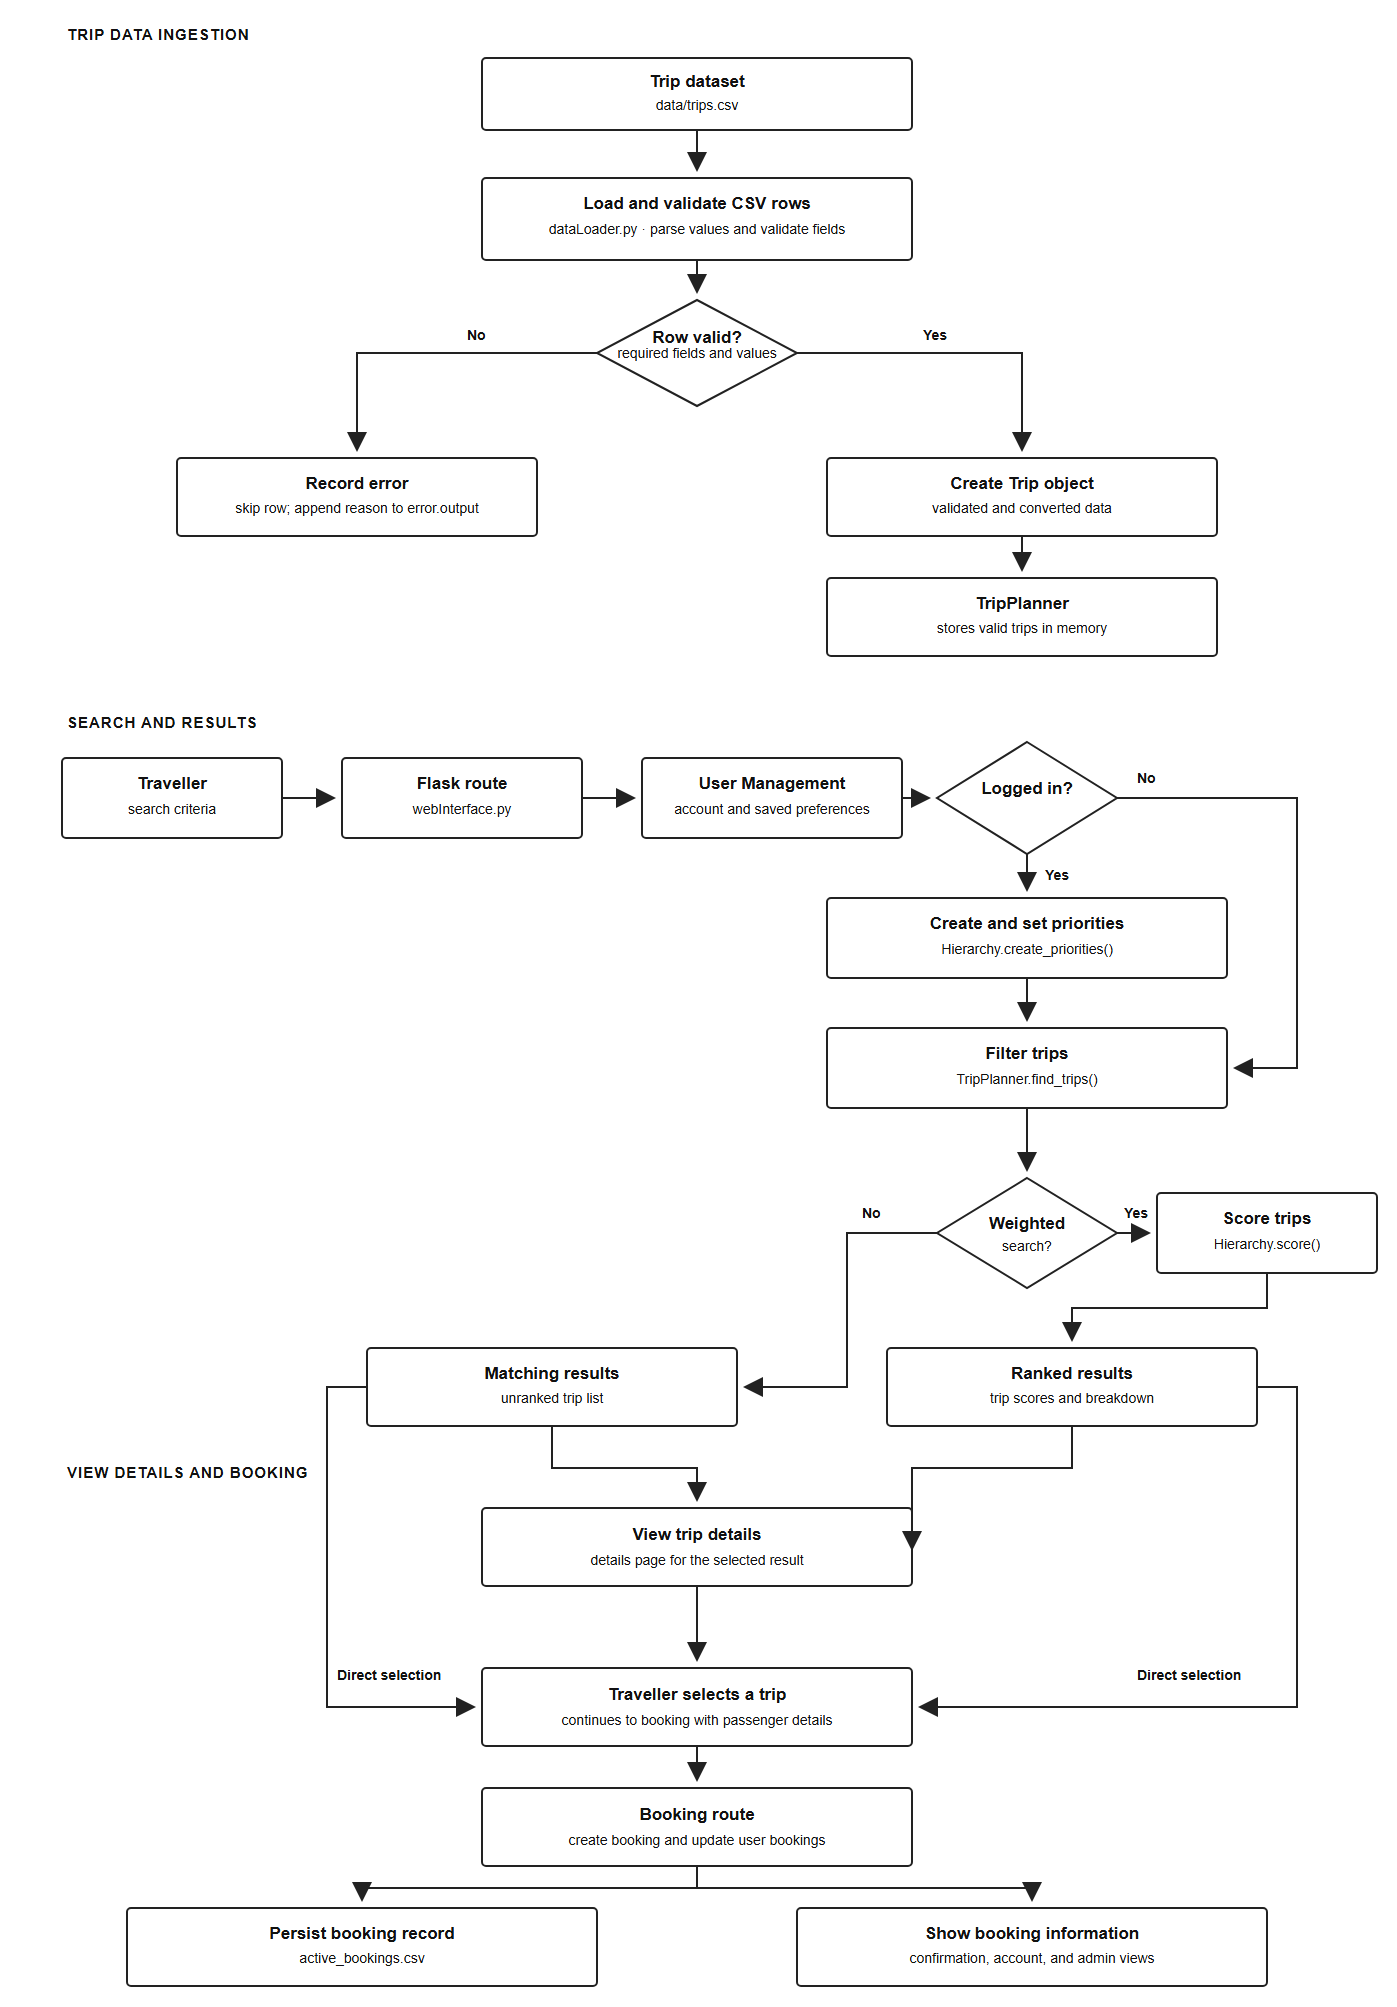
\includegraphics[width=\textwidth,height=0.82\textheight,keepaspectratio]
{../data/BusBidder_Data_Flow.png}
\caption{BusBidder data flow from trip ingestion through ranking and booking.}
\label{fig:architecture}
\end{figure}
\clearpage

\subsubsection{Trip Data Ingestion and Storage}
The \texttt{dataLoader.py} loads trip data from the file \texttt{data/trips.csv} and validates it row by row rejecting and reporting failed 
imports with reasoning before they are converted into \texttt{Trip} objects. The file \texttt{tripsService.py} then manages the storage of \texttt{Trip} objects, 
and is then used for querying stored trips, and also exports booking information to external files.

\subsubsection{Priority Evaluation and Ranking System}
The module \texttt{priority.py} defines priority types, qualifiers, and evaluation methods; and determines Trip scoring into \texttt{scoreObject.py}.
The module \texttt{priorityHierarchy.py} manages priorities and their weights.

\subsubsection{User Management and Graphical Interface}
The class definitions in \texttt{user.py} handle the user account data and model, stores a users weighted priorities; and also establishes a definition of a \texttt{Booking} object.
The \texttt{webInterface.py} module runs the Flask application and exports failed data imports and reasoning to the external file \texttt{error.output}.
webInterface is responsible for hosting the service, and exposing the application routes and page rendering logic. It also handles user input, validating it and querying against it.
It's through this module that the user can create an account, log in, and save their priority hierarchy, search for trips, and have the system display a ranked list of results.
The user can select a trip to book, and the system will save the fare conditions associated with the booking information and tie it to a unique booking reference 
utilizing an incrementor and the offerID while updating the Trip data to reduce it's capacity.

Due to the decision to not include database logic, the module also handles the persistence of user data and bookings.

\subsection{Object-Oriented Design Decisions}
The use of separate modules in this design allows the ranking system to operate independently from the web interface, which allowed for better organization and maintainability.
Most OOP design decisions used in this project revolve around the priority evaluation and ranking system, the application's core.
Inheritance, composition, and dynamic behaviour are relevant to the project. In designing the priority system, implementing an abstract \texttt{EvaluationMethod}
to be overwritten by the \texttt{Binary} and \texttt{Comparative} Evaluations classes 
within the priority object allows Trip scoring to adapt to different priority types without changing the application model.
For dynamic behavior, a user has a priority hierarchy that can change it's priorities at runtime.

\newpage
\section{Data Management and Validation}
The dataset for this program is stored in a CSV file, with each row representing a trip and its associated attributes.
The columns include the following:
\begin{itemize}[nosep]
\item \texttt{offer\_id} Required
\item \texttt{company} Required
\item \texttt{destination} Required
\item \texttt{travel\_date} Required
\item \texttt{arrival\_date} Required
\item \texttt{departure\_time} Required
\item \texttt{arrival\_time} Required
\item \texttt{duration\_minutes} Required
\item \texttt{price\_euro} Required
\item \texttt{transfers} Required
\item \texttt{transfer\_via} Optional
\item \texttt{luggage\_allowance\_kg} Required
\item \texttt{changeable} Required
\item \texttt{refundable} Required
\item \texttt{available\_seats} Required
\item \texttt{customer\_rating} Required
\item \texttt{rating\_scale\_max} Required
\item \texttt{environmental\_measure\_kg\_co2e\_per\_passenger} Optional
\end{itemize}

The contents of the dataset are a collection of bus trip offers from 5 distinct companies, 
across 15 destinations and dates ranging from 11-03-2027 to 11-09-2027.

Each CSV row is checked: Ensures required ID exists, a valid company and destination are given based, valid dates/times are given for departure and arrival, valid values and ranges for numeric fields, valid boolean fields, and Optional environmental-impact data is parsed when present.
If the checks pass, the function converts the values to suitable Python datatypes and creates a \texttt{Trip} object. 
If any validation fails, the row is rejected and the reason for rejection is logged to an external file \texttt{error.output}.

In the dataset, there are a total of 125 Trips with 8 Trips being invalid.
The 8 invalid trips were rejected due to the following reasons:
\begin{itemize}[nosep]
  \item Invalid price data. Price is mandatory and can not be a negative value.
  \item Invalid trip destination.
  \item Invalid date given with a month of 13.
  \item Arrival Date occurs before the departure date.
  \item Invalid customer rating data.
  \item There needs to be at least 1 available seat for a trip to be valid.
  \item Negative number of transfers
\end{itemize}

\newpage
\section{Searching, Filtering, and Scoring Methodology}
\subsection{Searching and Filtering Trip data}
The \texttt{tripsService.py} module is responsible for searching and filtering the stored trip data. It provides methods to query trips based on user-defined criteria,
Based on all available fields in data.
None of the parameters are required, allowing queries to be general or specific.
If no options are given, \texttt{tripsService.py} returns all trips in the dataset.
The User is able to make these queries through the web interface's Search page. 
From here specified filters are applied, and any trip that doesn't meet the criteria is excluded from the results.
It's in this Search form, that we create "hard constraints".

\subsection{Weighted Ranking Methodology}
For the implementation of a "soft constraint" we use the weighted ranking system to score and rank trips based on a user's preferences.
Assume a user has the following Trip priorities:
Price, Flexibility, Low transfers, short duration, Departure time after 17:00. We establish a structure that has 100 points and allow them to rank each prioritiy
in respect to a percentage of those points. 

In this example:
\begin{itemize}
  \item Price 37
  \item Flexibility 26
  \item Low transfers 19
  \item Short duration 11
  \item Departure time after 17:00 7
\end{itemize}
With this hierarchy we see two things: some need a comparison to determine their quality (i.e. what's a lower price in this context), and others are measured binarily.

For demonstrative purposes consider the following data:
\begin{table}[H]
\centering
\scriptsize
\setlength{\tabcolsep}{3pt}
\begin{tabular}{llccrccc}
\toprule
Company & Destination & \shortstack{Departure\\time}
& \shortstack{Duration\\(min)} & \shortstack{Price\\(EUR)}
& Transfers & Changeable & Refundable \\
\midrule
Camino Express & Barcelona & 15:15 & 399 & 89.64 & 0 & FALSE & FALSE \\
CostaLink & Barcelona & 13:30 & 484 & 60.25 & 0 & FALSE & TRUE \\
VerdeBus & Barcelona & 11:00 & 513 & 63.56 & 0 & FALSE & FALSE \\
NocheVia & Barcelona & 20:15 & 617 & 53.40 & 1 & TRUE & FALSE \\
NocheVia & Barcelona & 21:15 & 623 & 57.22 & 1 & FALSE & TRUE \\
\bottomrule
\end{tabular}
\caption{Example bus journeys to Barcelona.}
\label{tab:barcelona-trips}
\end{table}

If we determine minimums and maximums for price, transfers, and durations of our data, we can utilize the min max normalization formula to determine the share of its weighted points a priority is awarded.
For clarification: the trip with the lowest price should be given 37 of the 37 points; the average be given 18.5; and the most expensive be given 0

With this Trip data, we have:

- max price of 89.64 and a min of 53.40

- trip duration max: 623 and min: 399

- transfers max: 1 and min: 0

For actually scoring we use: $$X_{norm} = \frac{X - X_{min}}{X_{max} - X_{min}}$$. The new problem here is it isn't universal: A low Price is good, but a low customer rating isn't. For fields where lower values are better we can take the 1 - the normalization to get an appropriate scale.

Binary priorities award full points when criteria are met, such as a departure after a specified time.
Flexibility is a complicated Binary type because in this implementation we combine Refundable and changeable, but we can set it as 60%/40% refundability to changeability, since refunds are more valuable than changability. 
with this framework, if a trip allows changes but not refunds it'd get 40% of the 26 points given.

\subsubsection{Example scoring}
Trip 1:
- Price: $$X_{price} = 1 - \left(\frac{89.64 - 53.40}{89.64 - 53.40}\right) = 0$$

- Flexibility: Trip has no refunds or changability so $$0.6\left( 0 \right) + 0.4\left( 0 \right) = 0$$

- Transfers: No transfers $$X_{transfers} = 1 - \left( \frac{0 - 0}{1 - 0} \right) = 1$$ Transfers: 19 points

- Duration: This has the shortest duration $$X_{duration} = 1 - \left(\frac{399 - 399}{623 - 399} \right) = 1$$ 11 points

- Departure time after 17:00: this trip departs at 15:15 so it doesn't meet this expectation: 0 points

Trip 1: point total = 30 / 100 Meaning this trip isn't a great fit.

Doing this for all 5 trips we get the following results:
\begin{table}[H]
\centering
\scriptsize
\setlength{\tabcolsep}{3pt}
\begin{tabular}{lrrrrrr}
\toprule
Company & Price & Flexibility & Transfers & Duration & Departure Time & Total Score \\
\midrule
Camino Express & 0.00 & 0.00 & 19.00 & 11.00 & 0.00 & 30.00 \\
CostaLink & 30.01 & 15.60 & 19.00 & 6.83 & 0.00 & 71.44 \\
VerdeBus & 26.62 & 0.00 & 19.00 & 5.40 & 0.00 & 51.02 \\
NocheVia & 37.00 & 10.40 & 0.00 & 0.29 & 7.00 & 54.69 \\
NocheVia & 33.10 & 15.60 & 0.00 & 0.00 & 7.00 & 55.70 \\
\bottomrule
\end{tabular}
\caption{Example bus journeys to Barcelona with their respective scores.}
\label{tab:barcelona-trips-scores}
\end{table}

The benefit of allowing the user to assign a customizable weight is that even if another user ranks those priorities
in the same order, different distributions produce different scores.

\subsubsection{Scoring Implementation in this program}
Utilizing the Web form in the \texttt{webInterface.py} module, the user can select their priorities and assign weights to them. This is portrayed as a pie chart.
Once the user submits their priority data, the system will validate the input and create a \texttt{PriorityHierarchy}
object. In \texttt{priority.py}, each priority receives a weight and, when needed, a \texttt{Qualifier} 
specifying the operator and value used to compare trip data during scoring for added context.
A good example of the qualifier is the 'departure time after 17:00' priority, the qualifier here has an operator of "Later than" and value 17:00. 
Each \texttt{Priority} Object has an attribute \texttt{PriorityType} which maps it to a given Trip attribute and designates a specific evaluation method.
The PriorityType is an Enum that's used to determine which evaluation method to use for a given priority.
We established two evaluation methods, Binary and Comparative, these programatically distinguish what we manually did in the previous section

\newpage
\section{Web Interface and Booking Functionality}
We decided to utilize Flask and Jinja web interface for user interaction. the Flask Application structure uses python
Decorator functions such as \texttt{@app.route("/booking", methods=["GET", "POST"])} to route the user.
This allows a user to customize the flow through the application.
The application has several routes for the user to navigate:
\begin{itemize}
\item An index page that allows navigation to most other pages.
\item A login/registration page that lets a user register an account or log in to an existing one. Once valid account data is entered, the user is redirected to a profile management page. New accounts are saved on the server and in \texttt{registered\_users.csv}.
\item A profile management page that allows a user to change account information and site theme, set and weigh priorities, and view details of booked trips.
\item A quick search page, available from the index page after login, where the user can specify ticket quantity, destination, and date or date range. The application uses the user's priorities to show up to six matching trips.
\item A search page that allows any user to find trips using the search fields. Logged-in users can also rank the results. From the results, users can open a trip details page or go directly to booking.
\item A details page that displays information about a trip. For logged-in users, it also displays the trip's scoring breakdown and explains its score.
\item A booking page that displays trip information for confirmation. The user can select a number of seats up to the available capacity, enter passenger names, and submit the booking. Bookings are saved on the server and exported to \texttt{active\_bookings.csv}.
\end{itemize}

These are HTML Flask pages using Jinja Scriptlets which allowed us to easily acess python objects and data for display.
All of these pages exist in the \texttt{./templates} directory, and their styling and JavaScript files are in \texttt{./static} directory.

\newpage
\section{Testing and Experimental Results}
The testing for this application uses Python's built in unittest modules.

\texttt{test\_dataLoader\_unittest.py} checks valid and invalid files, empty or non existant files, dates before today,
and whether invalid rows produce expected errors.
These tests utilize the error validation in the \texttt{dataLoader.py}'s data ingestion to catch all invalid rows
to cover invalid, boundary, and missing data-cases on data import and processing.

\texttt{test\_trip\_scoring\_unittest.py} checks priority weight limits, duplicate priorities, missing time qualifiers,
and checks that scores and breakdowns are produced.
Theses tests validate the application's scoring metrics and also verify that our weight-based scoring
can systemically rank trip data on a per user basis.
The final tests in this module validate that two different usesr with different priorities rank the test data in a different order.

\begin{figure}[H]
\centering
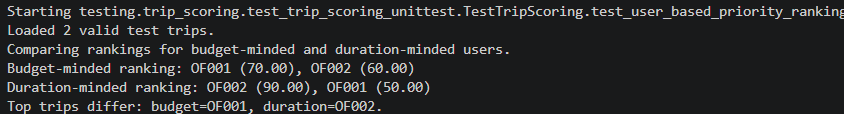
\includegraphics[width=\textwidth]{priority_top_scoring_trip_test_result.png}
\caption{Console output showing different top-ranked trips for two traveller priority profiles.}
\end{figure}

\begin{figure}[H]
\centering
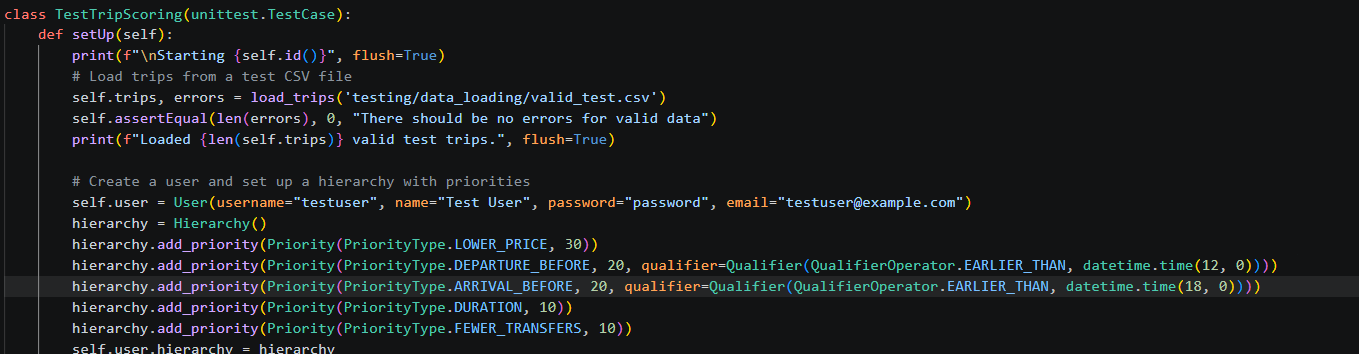
\includegraphics[width=\textwidth]{default_user_priority_test.png}
\caption{Unit test code showing the budget minded users priority weighting.}
\end{figure}

\begin{figure}[H]
\centering
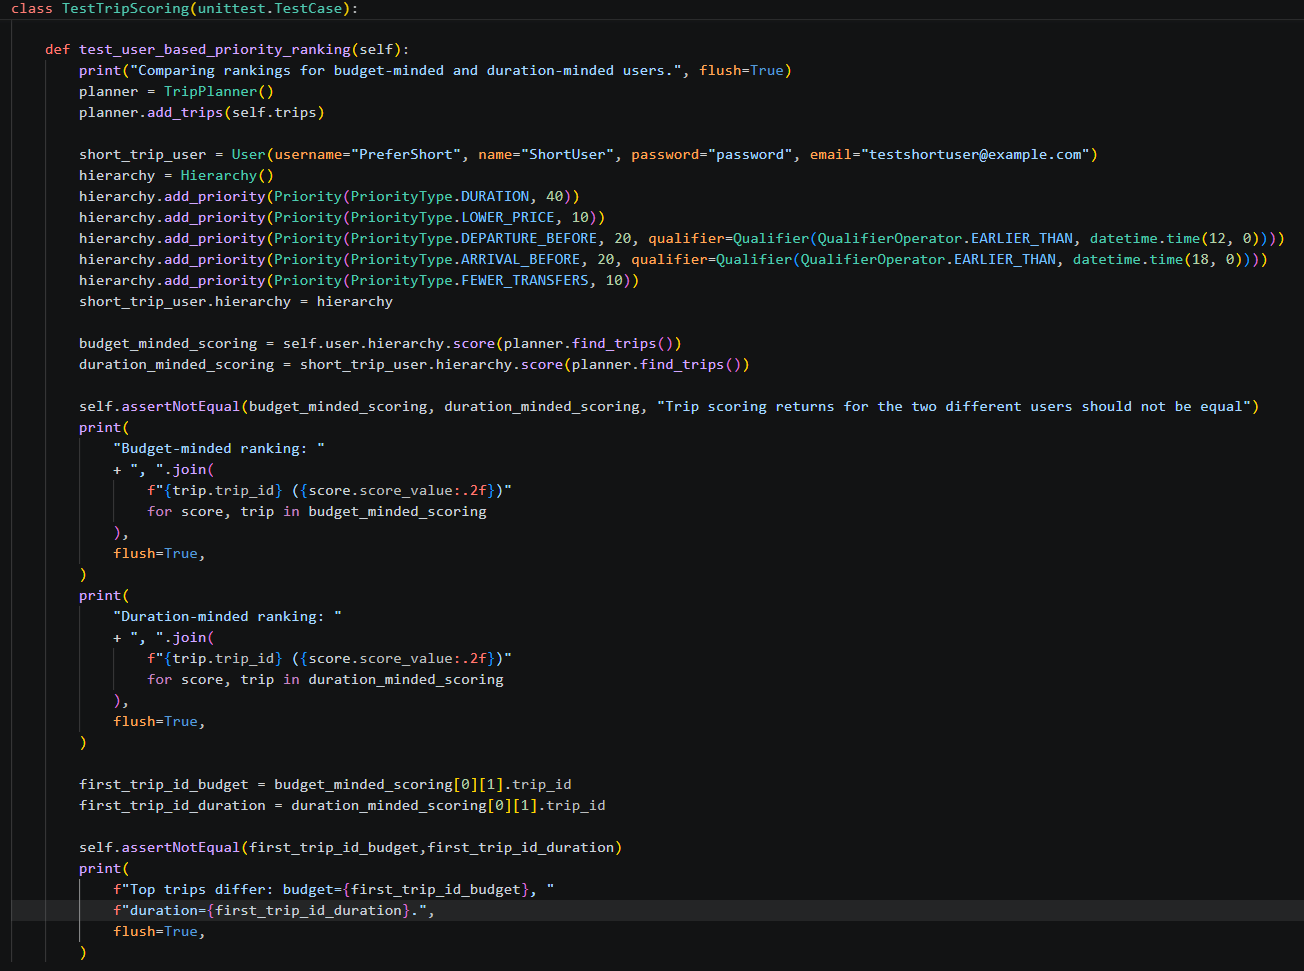
\includegraphics[width=\textwidth]{scoring_difference_code.png}
\caption{Unit test code comparing trip rankings for budget-minded and duration-minded users.}
\end{figure}

The ranking system is measured here for the same trips when given the context of the different user's priority weighting.
Not only is the first recommended trip for each user different; the relevance scores differ greatly considering
only the weight given to the duration and prices have changed.

\newpage
\section{Traveller Profile Comparisons}
We'll compare three traveller profiles, with a different theme for each user for readability.

  \begin{itemize}
  \item \textbf{Budget-focused traveller}: prioritises low price, departures after work at 18:00, and flexibility.
    \begin{figure}[H]
    \centering
    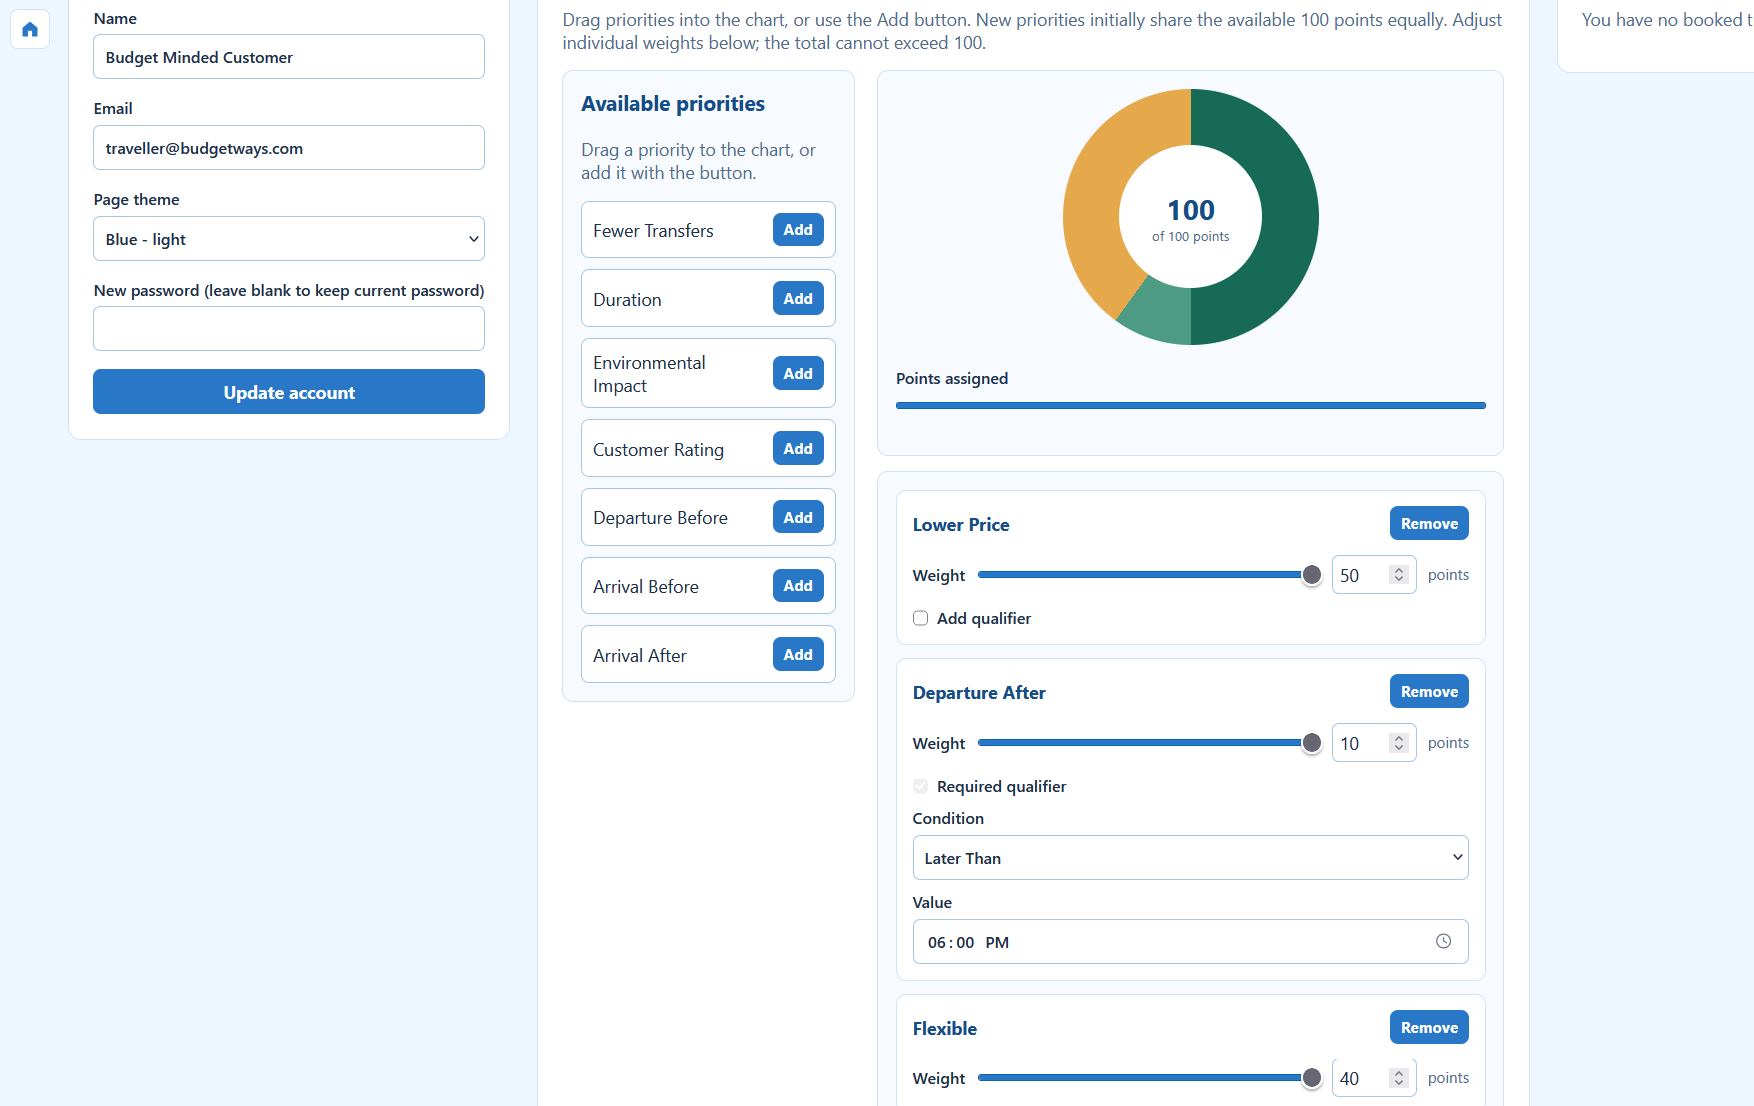
\includegraphics[width=\textwidth]{budget_priority_list.png}
    \caption{Priorities and weights of the Budget Minded user}
    \end{figure}
  \item \textbf{Business traveller}: prioritises time efficiency, quality, and fewer transfers.
    \begin{figure}[H]
    \centering
    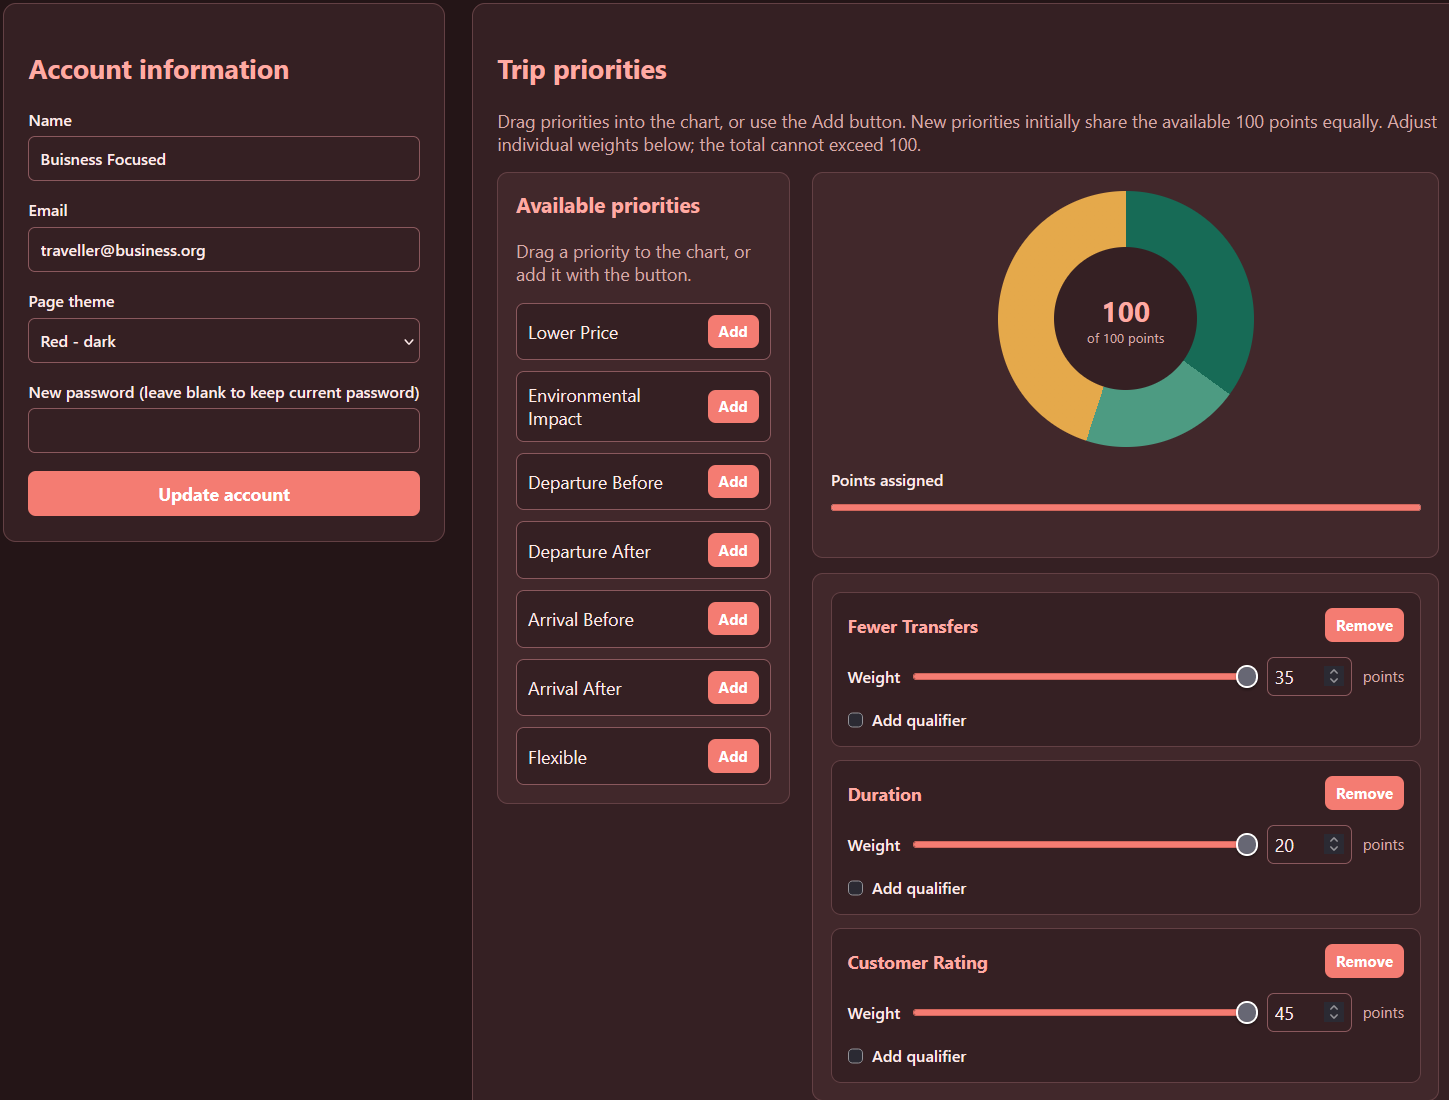
\includegraphics[width=\textwidth]{business_priorities.png}
    \caption{Priorities and weights of the Business user}
    \end{figure}
  \item \textbf{Environmental-focused tourist}: prioritises lower Carbon impact, shorter duration, and fewer transfers.
    \begin{figure}[H]
    \centering
    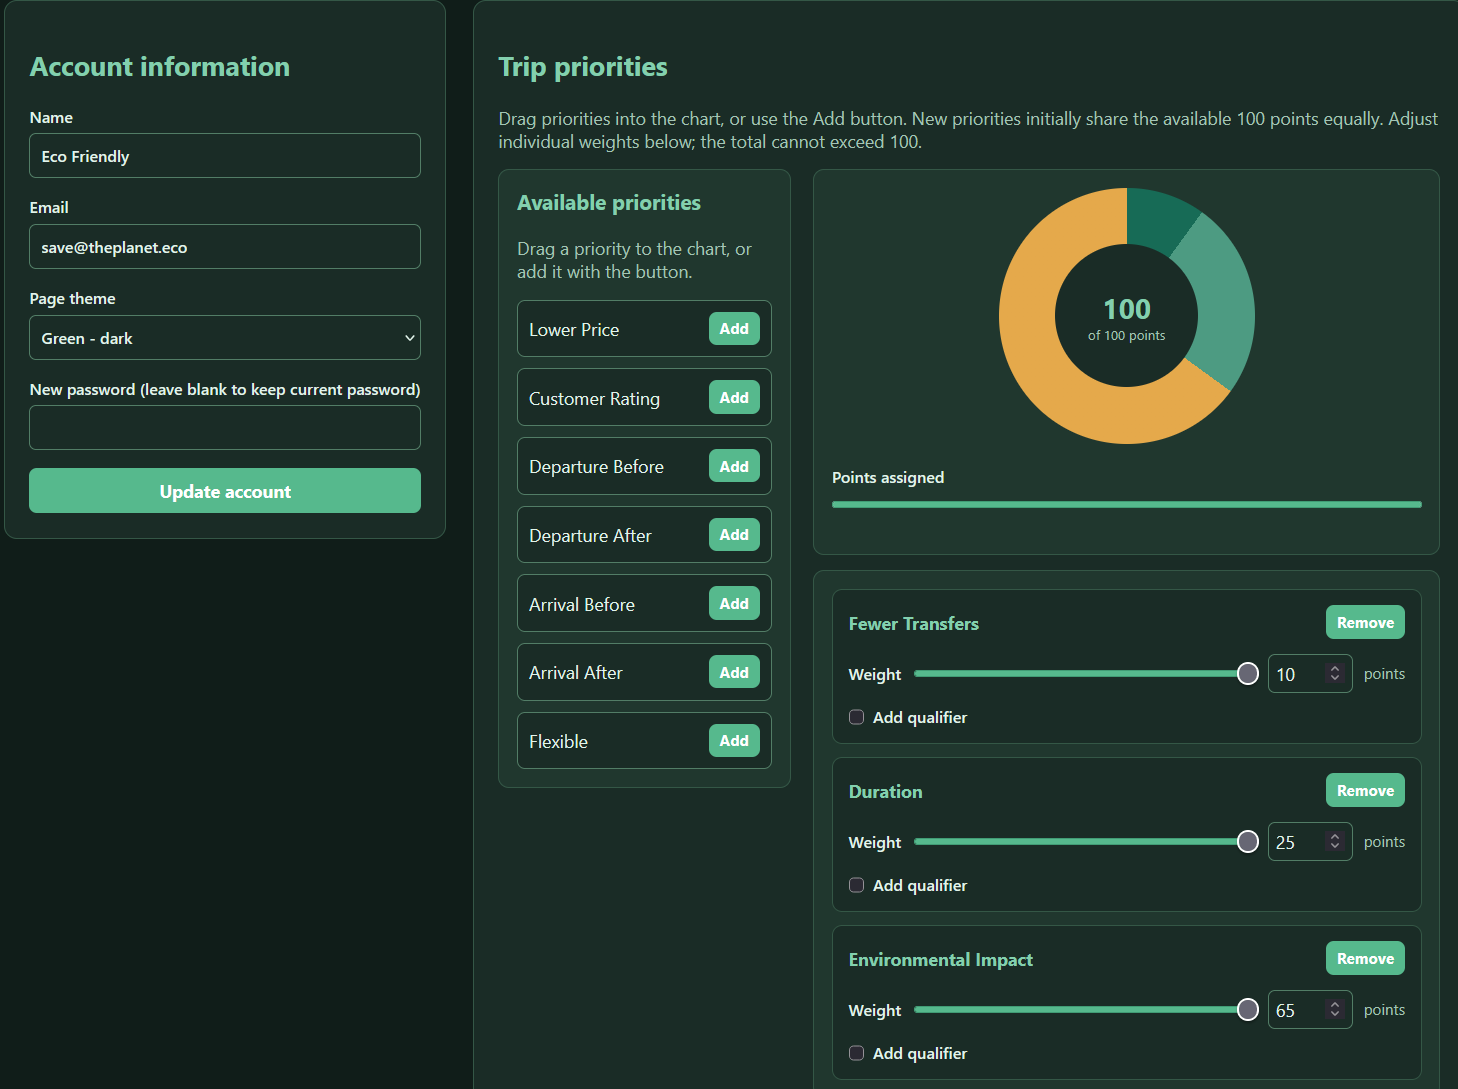
\includegraphics[width=\textwidth]{ecominded_priorities.png}
    \caption{Priorities and weights of the Environmental minded user}
    \end{figure}
  \end{itemize}

For this demonstration, a query is made for trips going anywhere (can be done by not selecting a destination or pressing control while you select destinations)
with departure dates ranging from 11-04-2027 to 11-07-2027. This should return 71 trips.

For each user we have different ranked results as seen below:

  \begin{figure}[H]
  \centering
  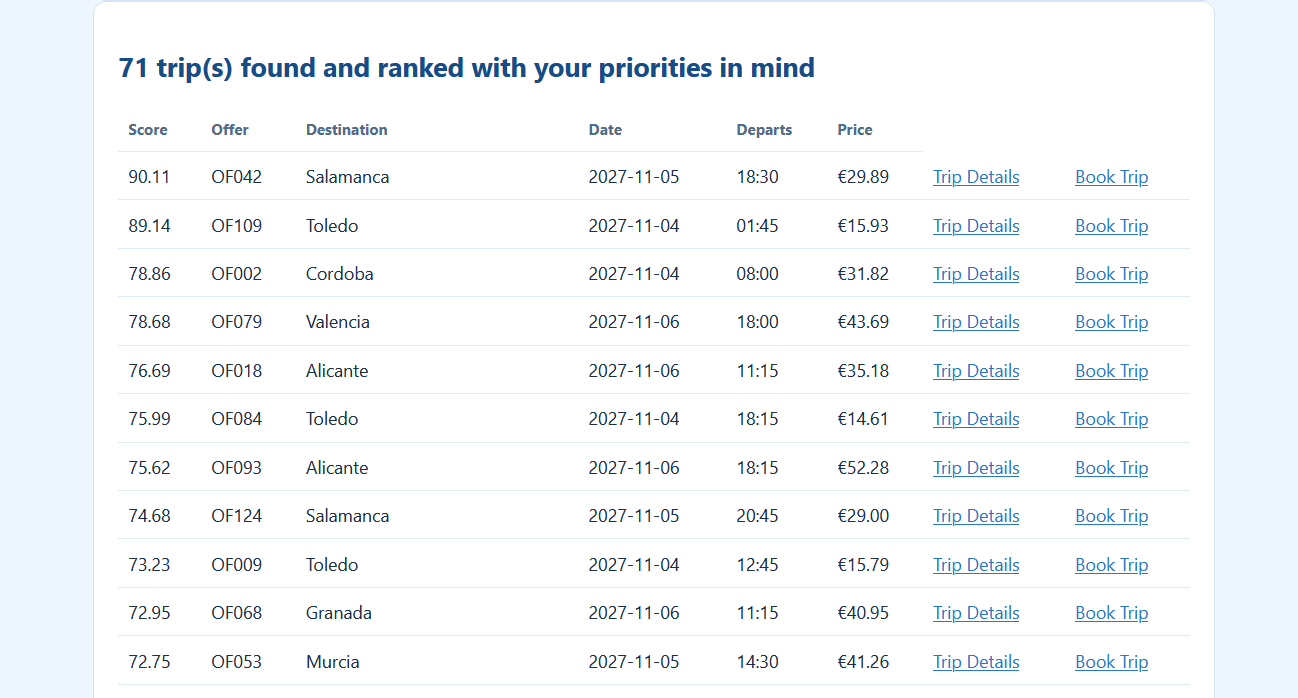
\includegraphics[width=\textwidth]{budget_results.png}
  \caption{Top recommendations of the Budget Minded user}
  \end{figure}

  \begin{figure}[H]
  \centering
  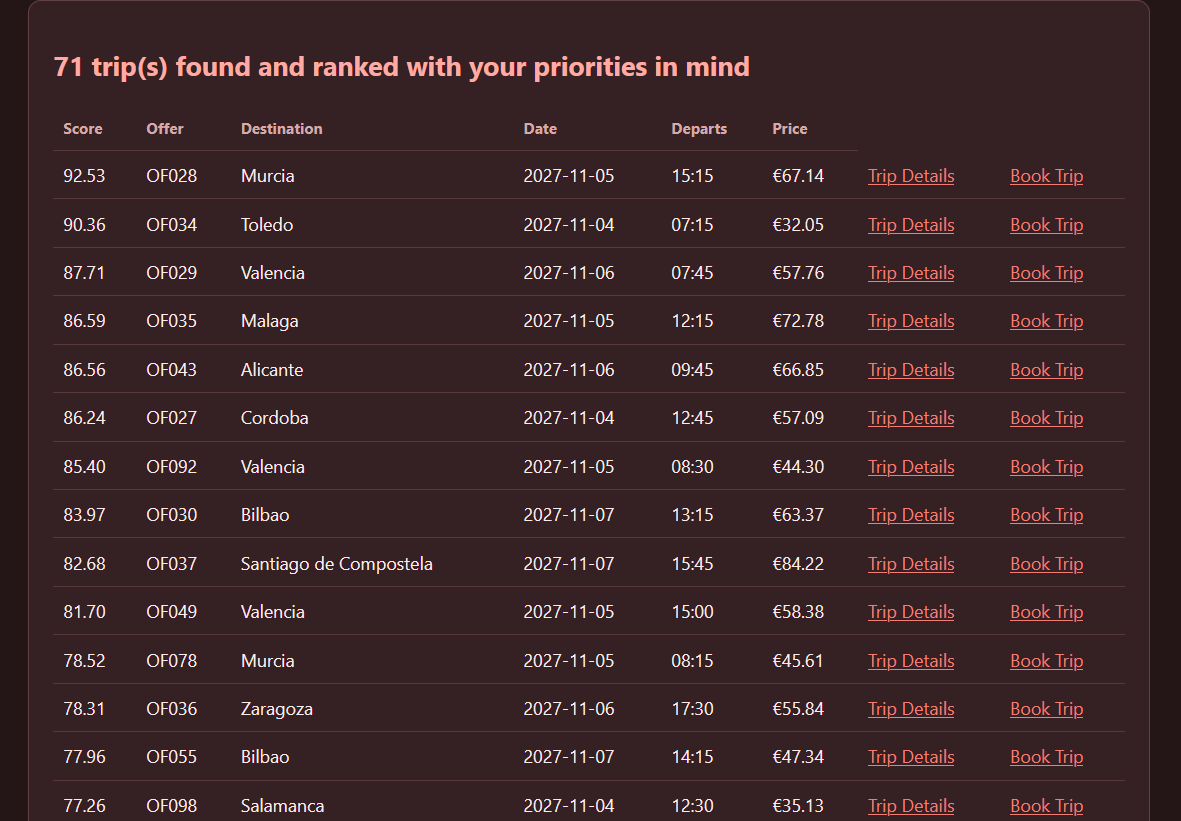
\includegraphics[width=\textwidth]{business_results.png}
  \caption{Top recommendations of the Business user}
  \end{figure}

  \begin{figure}[H]
  \centering
  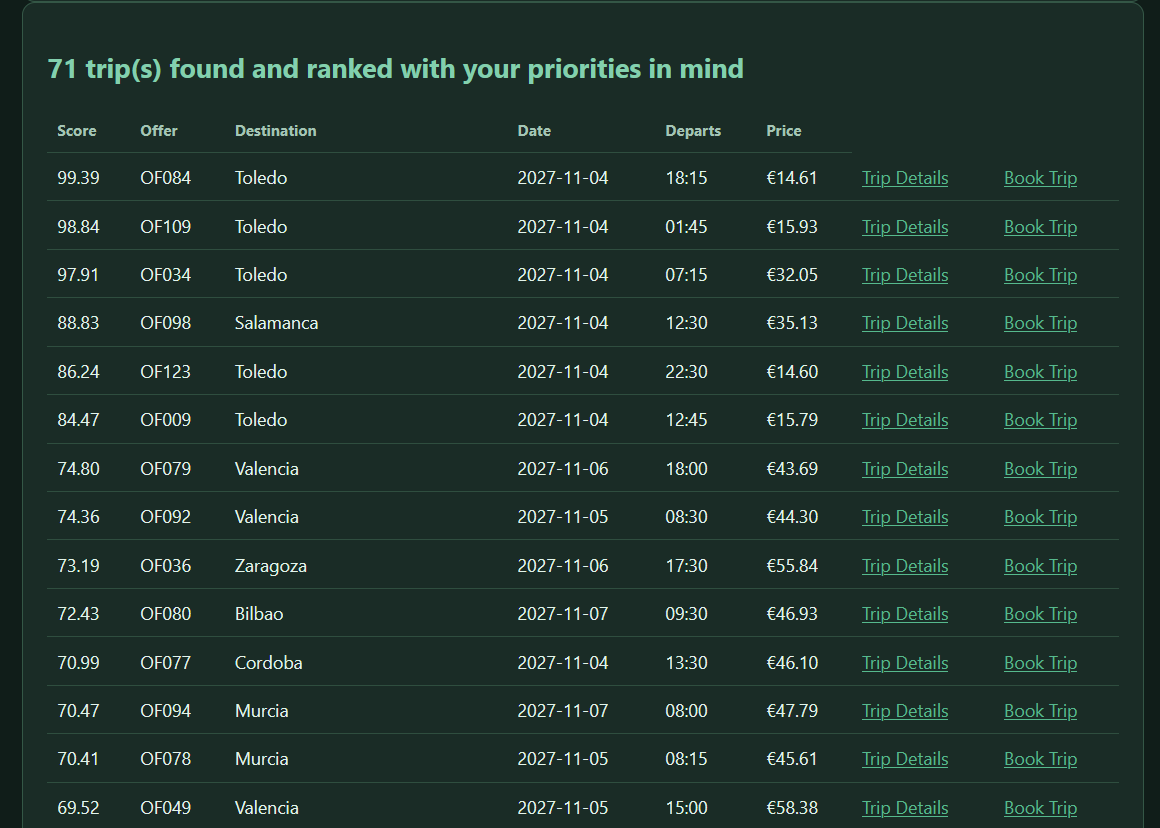
\includegraphics[width=\textwidth]{eco_results.png}
  \caption{Top recommendations of the Environmentally focused user}
  \end{figure}

Each user's recommendations have a unique order and scoring.
If we look into each users highest choice we can also see a break down of the scoring as well as all other trip information.

 \begin{figure}[H]
  \centering
  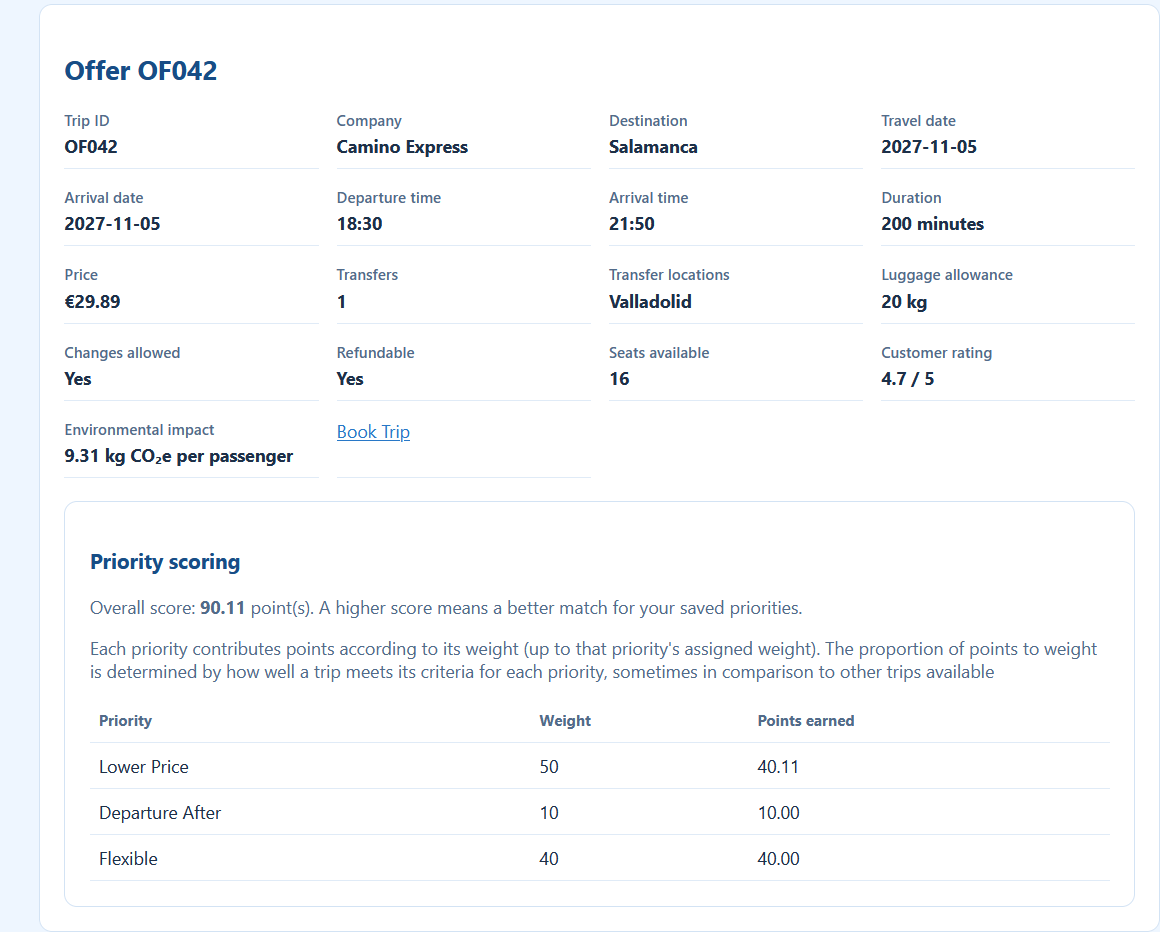
\includegraphics[width=\textwidth]{budget_no1_details.png}
  \caption{Top trip of the Budget Minded user}
  \end{figure}

  \begin{figure}[H]
  \centering
  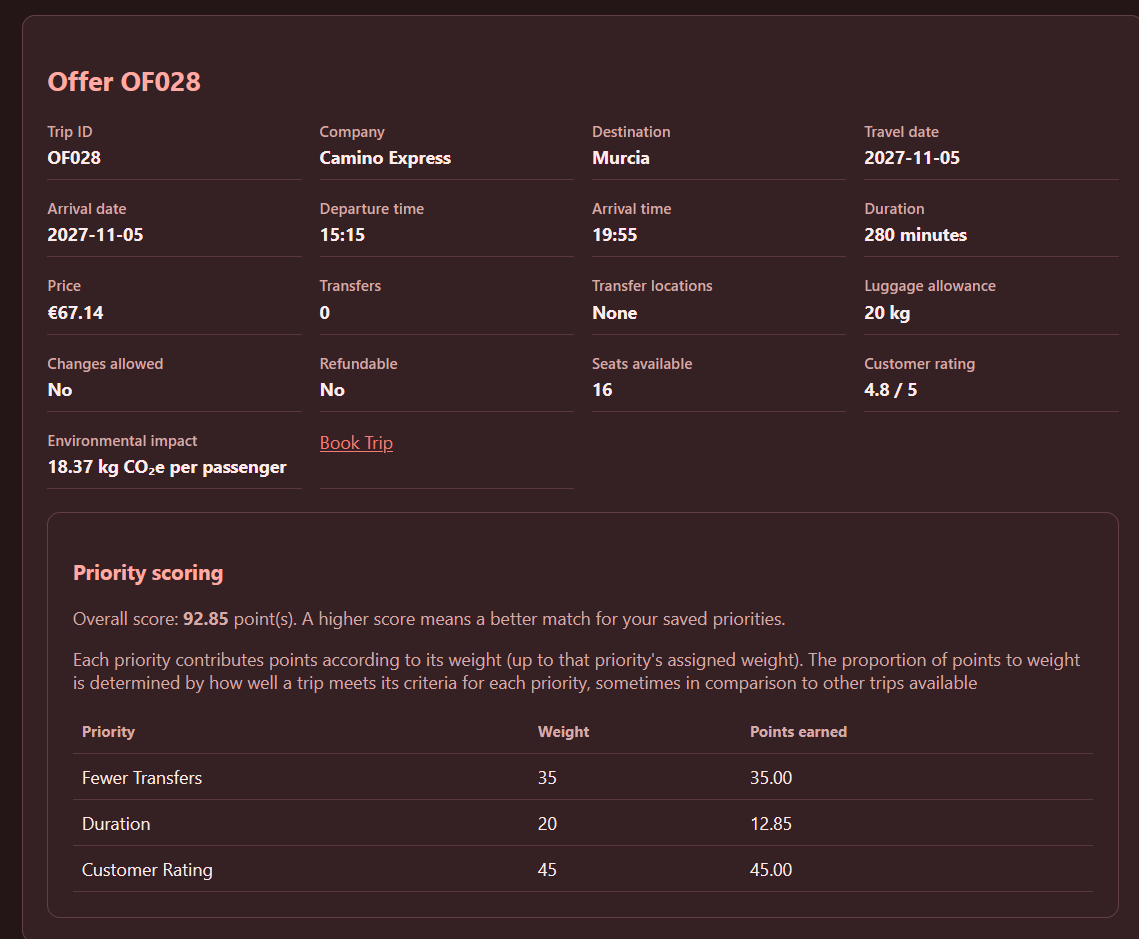
\includegraphics[width=\textwidth]{business_no1_details.png}
  \caption{Top trip of the Business user}
  \end{figure}

  \begin{figure}[H]
  \centering
  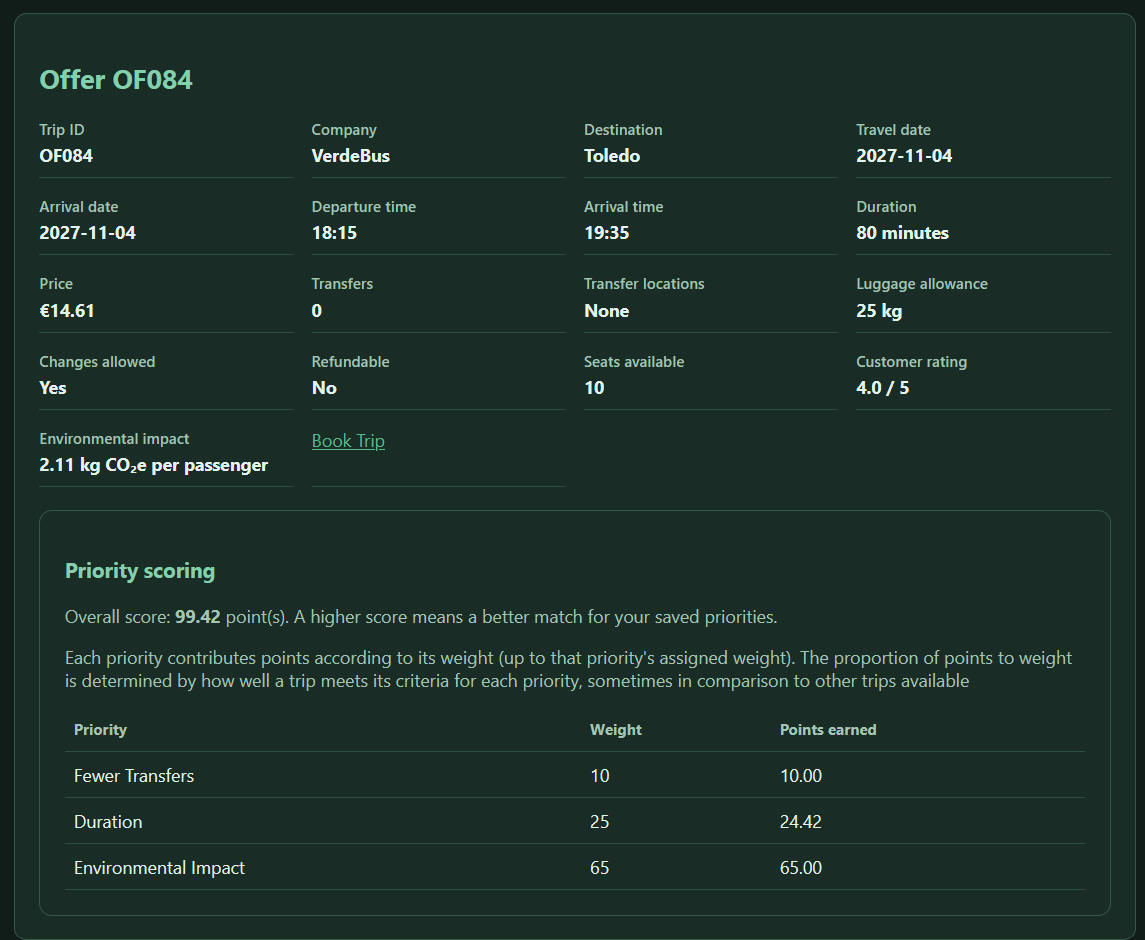
\includegraphics[width=\textwidth]{eco_no1_details.png}
  \caption{Top trip of the Environmentally focused user}
  \end{figure}

We can see that each of the user's top recommended trips have a score breakdown on how well it meets up with their specific priorities,
and they can tell how the trip aligns with their preferences in comparison to other trips. For instance when a comparitive score like
Environmental Impact, or Price recieves all points of its share, the user knows that it's the lowest of the trips in the offering.

In the case of the budget users highest rated trip, the user can tell from this details pane
that while it's only close to being the cheapest; it's  also flexible, and departs after the work day. These factors push its score above the cheapest trip.
Here we see the value in the design decision of adding this weighted scoring over showing the cheapest trip available.

\newpage
\section{Critical Evaluation and Limitations}
As a basis; for this kind of problem and use case, a web interface makes the most sense
as it's an intuitive means for a user to browse trips and details and store information about them selves. It's a familiar format and as such requires
little explanation on how to use the program. 
Secondly the decision to take certain priorities a user holds and have the user to select and weigh them allows
for a more personalized service. As mentioned above, A user would be able to find appropriate trips on their own with a table that allows them to filter on things
like Prices, customer rating, etc. on a scale of low to high or High to low; however,
this approach only takes one or two things into consideration. The weighted approach as demonstrates a more indepth application that can show a trip
that aligns across all of areas a user cares about. This applications design implementation also is modularized enough that future modifications
would be trivial to add. For example, if we wanted to be able to add a new priority; the framework exists in such a state that it'd only need to be
updated in the priority objects code and then in the front end. Everything else that interacts with this data is generalized enough that it'll accept new data
if structured in those two places.

This application is, however, limited in a few aspects. Because we're reading in data from a fixed CSV file, our breadth of trip complexity is limited to what's
present. It'll also eventually be unusable due to Dates being passed. The scoring also leaves its results as a floating value that
can technically lead to ties, but it was intentionally decided that a floating point value of 2 decimal places would be sufficient scoring. The user should be
able to look at two trips with the same score and be able to use the extra information and decide what would their tie breaker should be.
Accounting for that programmatically would weigh down the user experience and make possibly incorrect assumptions. 
We also are consider in its current state, the established priority system may miss something that matters to a 
user. While this could be remedied by adding more and more priorities to the list,
it was decided for this project that the given priorities would be sufficient also considering the user could manually query the data with anything else that data
in a file may contain.

The scoring and normalization are robust enough, but some decisions made don't seem to fit the current data set.
A prime example of this is that we currently score a priority of low number of transfers in a comparative evaluation methodology.
In our dataset, trips only have 0 or 1 transfers which would work in a binary evaluation; however, it was a measured decision that it was possible
for someone running the program to feed the application data with many transfers, and in that case a binary approach would be insufficient.

Allowing users to set their own priorities can introduce bias in the rankings. For example, a user may value low carbon impact more than low price. 
If trips have similar carbon impacts but one is an unusually cheap outlier, min-max normalization can compress the price scores of the other trips. 
This may cause price to outweigh small differences in carbon impact and change the ranking.

One alternative is to normalize against the overall distribution rather than the observed minimum and maximum. 
However, that would reduce the influence of outliers, which some users may value. There is no universally correct approach; 
this implementation retains outlier sensitivity and as such is how we decided to keep it.

\newpage
\section{AI Declaration of Use}
The CSV file \texttt{data/trips.csv} that contains the data for our trips was populated using chatGPT. It was given the context of the companies
and the given locations. This felt acceptable because it allowed me to quickly generate 125 realistic trip offers and aside from deciding what kind of 
data would be present, coming up with valid seeming data at this scale seemed outside of the scope of the assignment.
Generated data was reviewed, manually modified where necessary for example in the date and time fields when they were not in the right format
for Python Date/Time object conversions.

I also utilized the coPilot AI built into VS code to help generate the templates of forms, style sheets, and javascript interactivity of the web pages used. Web development skills seemed 
out of scope for grading criteria, so this seemed appropriate. I did manually implement the Jinja scriptlet tags that allowed for a cleaner 
interaction between the flask interface to python, and the html based web pages. 

Vs Code's auto code complete was also used to quickly build class and function declarations, and in the tripService.py 
initalizer function because it was only tedius attribute setting to parameter values   
but all other logic and design decisions made in the application were made without the aid of the AI tools present in the IDE

AI was used to comb through report to change some words like "it is", "can not", "is not" to their contraction equivalent and remove extra and trailing spaces to clean up report,
but wording is all still and sentence structure is all still Human.
\end{document}
